\section{Représentation des données}
\setcounter{exemple}{0}

\begin{exemplebox}
    Réalisons une enquête dans la classe : "Sur combien de réseaux sociaux
    avez-vous un compte ?"
    \vspace{5cm}
\end{exemplebox}

\subsection{Représentation en tableau}
\begin{remarquebox}
    La représentation brute des résultats n'est guère exploitable, il est 
    donc usuel de regrouper les résultats par valeurs identiques dans un tableau
    appelé \hlb{tableau des effectifs}.
\end{remarquebox}

\begin{exempleboxsuite}
    \begin{itemize}[label=\textbullet]
    \item Pour l'exemple 1 la variable est dite \hlb{quantitative} (les réponses
        sont des quantités) \\

        \begin{tabular}{|c|c|c|c|c|}
            \hline
            \bb{Nombre de réseaux} &
            \answer{1} & \answer{2} & \answer{3} & \answer{4} \\
            \hline
            \bb{Nombre d'élèves (= Effectif)} &
            \answer{3} & \answer{8} & \answer{10} & \answer{4} \\
            \hline
        \end{tabular}

        \vspace{5pt}

    \item Pour l'exemple 2, la variable est \hlb{qualitative} (les réponses ne sont
        pas des quantités) \\

        \begin{tabular}{|c|c|c|c|c|c|}
            \hline
            \bb{App préférée} & Instagram & Tiktok & Facebook & Snapchat
            & Autre \\
            \hline
            \bb{Effectif} &
            \answer{8} & \answer{7} & \answer{3} & \answer{5} & \answer{2} \\
            \hline
        \end{tabular}

    \end{itemize}
\end{exempleboxsuite}

\subsection{Représentation graphique : diagramme en barres}
\begin{definitionbox}
    Un \hlb{diagramme en barres} (aussi appelé \hlb{diagramme en bâtons}) est un
    graphique qui à chaque valeur, associe un bâton (segment) de
    \bb{hauteur proportionnelle} à l'effectif correspondant.
\end{definitionbox}

\begin{center}
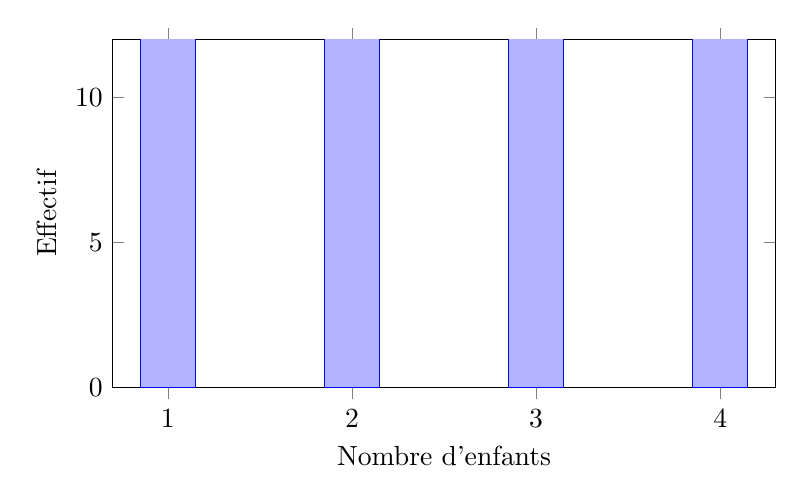
\begin{tikzpicture}
\begin{axis}[
    ybar,
    xlabel={Nombre d'enfants},
    ylabel={Effectif},
    ymin=0,
    ymax=12,
    xtick={1,2,3,4},
    bar width=20pt,
    width=10cm,
    height=6cm,
]
\addplot coordinates {
    (1,\graphanswer{71})
    (2,\graphanswer{305})
    (3,\graphanswer{117})
    (4,\graphanswer{92})};
\end{axis}
\end{tikzpicture}
\end{center}


\subsection{Représentation graphique : diagramme circulaire}
\begin{definitionbox}
    Un \hlb{diagramme circulaire} (aussi appelé \hlb{diagramme en camembert}) est un
    graphique qui à chaque valeur, associe un secteur de
    \bb{angle proportionnel} à l'effectif correspondant. \\

    Par exemple, le diagramme circulaire représentant la répartition des animaux à la SPA pourrait-être:

    \begin{center}
    \begin{tikzpicture}
    \pie{
        33/Chat,
        60/Chien,
        7/Cochon d'inde
    }
    \end{tikzpicture}
    \end{center}


\end{definitionbox}
\begin{exempleboxsuite}
    Toujours dans le cas de notre premier exemple, le diagramme circulaire de la
    répartition des élèves selon leur moyen de locomotion est : 
    \begin{center}
    \begin{tikzpicture}
    \pie{
        12.14/Deux roues,
        52.14/Bus,
        20/À pied,
        15.72/Voiture
    }
    \end{tikzpicture}
    \end{center}

\end{exempleboxsuite}


\subsection{Pourquoi utiliser des représentations graphiques différentes ?}
\begin{remarquebox}
    En fonction des données que l'on souhaite analyser, de l'information
    que l'on souhaite extraire, il peut être plus judicieux d'utiliser un
    diagramme plutôt qu'un autre. \\

    Le domaine des statistiques est l'un des domaines les plus riches de
    mathématiques et trouve de nombreuses applications dans le quotidien. Il est
    utilisé par les scientifiques, \bb{mais pas que !}. \\

    En effet, au cours de ta vie tu feras face à de nombreuses situations où il
    te faudra analyser des statistiques. A toi de savoir comment les représenter
    pour comprendre l'information. \\

    Prenons notre exemple précédent.
\end{remarquebox}

\begin{exempleboxsuite}
    Si je souhaite connaitre le \bb{nombre} d'élèves venant au collège à pied,
    autrement dit \answer{l'effectif} des élèves venant au collège à pied, il
    vaut mieux utiliser \answer{un diagramme à batons}. En effet il nous
    donne \bb{directement} accès à cette information ! C'est beaucoup plus compliqué
    en utilant un \answer{diagramme circulaire}. \\

    En revanche si je souhaite connaître la \bb{proportion} d'élève venant à
    pied, autrement dit la \answer{fréquence} des élèves venant à pied, il est plus
    judicieux d'utiliser un \answer{diagramme circulaire}. En effet il nous
    donne \bb{directement} accès à cette information ! C'est beaucoup plus compliqué
    en utilant un \answer{diagramme à bâtons}. \\
\end{exempleboxsuite}
